
\documentclass[submit,techreq]{ipsj}
%\documentclass[submit,draft]{ipsj}


\usepackage[dvips]{graphicx}
\usepackage{latexsym}

\def\Underline{\setbox0\hbox\bgroup\let\\\endUnderline}
\def\endUnderline{\vphantom{y}\egroup\smash{\underline{\box0}}\\}
\def\|{\verb|}

\setcounter{巻数}{53}
\setcounter{号数}{10}
\setcounter{page}{1}

\受付{2011}{11}{4}
%\再受付{2011}{7}{16}   %省略可能
%\再再受付{2011}{7}{20} %省略可能
\採録{2011}{12}{1}

\begin{document}


\title{語の出現パターンと意味関係分析を用いた\\
Webからのタスク検索}

\etitle{Subtask search}

\affiliate{IPSJ}{情報処理学会\\
IPSJ,Chiyoda,Tokyo 101--0062,Japan}


\paffiliate{KU}{京都大学\\
Kyoto Uniersity}



\author{加藤 龍}{Ryo Kato}{IKU}[r.kato@dl.kuis.kyoto-u.ac.jp]
\author{大島 裕明}{Hiroaki Ohshima}{IPSJ}[ohshima@dl.kuis.kyoto-u.ac.jp]
\author{山本 岳洋}{Takehiro Yamamoto}{IPSJ,KU}[yamamot@dl.kuis.kyoto-u.ac.jp]
\author{田中 克己}{Katsumi Tanaka}{IPSJ,KU}[ktanaka@i.kyoto-u.ac.jp]
\author{加藤 誠}{Makoto P. Kato}{IPSJ,KU}[kato@dl.kuis.kyoto-u.ac.jp]

\begin{abstract}
本研究では,クエリとしてタスクが与えられた際に,そのタスクを達成するために必要なサブタスク群をWebから発見する手法を提案する. 提案手法では,動詞の含意関係や逆意関係にもとづいたルールによりクエリの変換を行う. 変換したクエリでWeb検索を行う. 得られたページから,タスク特有の言語パターンを用いて,サブタスク候補となるフレーズを発見する. 
\end{abstract}

\begin{jkeyword}
タスク検索
\end{jkeyword}

\begin{eabstract}
This study is about subtask search.
\end{eabstract}

\begin{ekeyword}
Task search
\end{ekeyword}

\maketitle

%1
\section{動機}

誕生以来,Webには多様な資料が集積され続けている. 情報をどう走査,発見し,取捨選択するか,様々な方向からのアプローチがなされている. 
現在,いくつもの検索エンジンが実用化され,Webを舞台に情報発見や集約を行っている. だが,Webにおける情報検索は,いまだ多くの問題を抱えている. 
そのうちの一つとして,目的を達成する手段を発見したいとき,できるだけ多くの方法を探そうとしても意外と見つけられないことがあげられる.


なにかを成し遂げたいが,どうすれば成功するかわからないとき,Web検索を使って実現方法を考える行為がよく行われている. たとえば「花粉症対策をする方法」をクエリに検索することで,立体マスクをつける」や「アレロック錠剤を飲む」を発見することができる. だが,そうして発見できた「花粉対策をする方法」を採用すべきなのか,簡単にはわからない. まだ発見できていない「花粉対策をする方法」のほうがよいかもしれないからだ.


こうした状況では,多くのユーザーは「タスクを遂行するためにどんな方法があるか」をできるだけ多く発見するサブタスク検索を求める. 多様な答えが得られた段階で,初めて,安心して各方法を比較したり,自分にとって最適な方法を考えることができるようになる.

サブタスク検索の例を説明する.たとえば「花粉症対策をする」というクエリを入力すると,出力として


\begin{itemize}
\item \|立体マスクをつける|
\item \|アレロック錠剤を飲む|
\item \|医師の診断を受ける|
\item \|植物に近寄らない|
\end{itemize}


といったように,複数の異なった選択肢を複数発見する.これがサブタスク検索の例である. このように,できるだけ多くの手法を探そうとする検索は現在の一般的な検索エンジンでは困難である. 花粉症対策の方法は非常に多様であり,高くランクづけされたページであっても花粉症対策の方法のごく一部を含んでいるにすぎない. また高くランクづけされたページ同士は内容が重複していることが多く,高ランクのページを見て回っても,発見できる花粉症対策の方法の数は増えない。

このようなサブタスク検索が実用的なレベルに達すれば、\figref{fig:future_app}のように、 現在の検索エンジンが実装しているサジェスト機能にサブタスク検索を組み込むといった応用が考えられる。

\begin{figure}[tb]
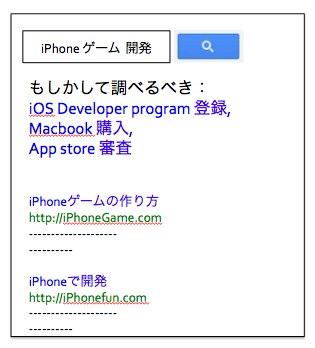
\includegraphics[width=6cm, bb=0 0 250 419]{future_app.jpg}
\caption{アプリケーションの例}
\ecaption{Application.}
\label{fig:future_app}
\end{figure}


タスク検索は、Web検索のなかでもかなりの割合を占めている。サブタスク検索を実現することは、Webでの検索体験を向上させる点で非常に有意義である。

本稿では可能な限り多様な方法をWebから発見する手法を提案し,評価する.


%2
\section{関連研究}

\begin{itemize}
\item \|サブゴールのクラスタリング|
\item \||
\item \|タスクとは,遂行すると,目的の一部あるいは全部を達成したことになるアクションである|
\item \|サブタスクとは,タスク同士の関係に着目したとき,「遂行するともう一方のタスクの一部を遂行したことになる行動」である. このとき「もう一方のタスク」はスーパータスクである|
\end{itemize}

\cite{yamatake}において,広告を用いたクエリクラスタリングが試みられている. タスク遂行のための,複雑な検索の手順を研究したものとして\cite{hassan}がある. また田麦らによるタスク遂行のためショッピングサイトなどサービスを提供するページを発見する研究\cite{tamugi}がある.

%3
\section{タスク関係の概要}
ある目的を達成するためにどのような順番でどのような行動を取るか考察する際,タスク,ゴール,アクションといった用語の定義が必要となる.


%3.1
\subsection{用語の定義}

本稿ではゴールを以下のように定義する.

\begin{itemize}
\item \|ゴールとは,目的の一部または全部を達成した状態である|
\item \|アクションとは,ある状態から別の状態に移行する行為である|
\end{itemize}

ゴールとアクションを図示すると\figref{fig:action_goal}のようになる。「花粉症対策している状態」がゴールであり、「花粉症対策をしていない状態」から「花粉症対策している状態」に移行する行為がアクションである。\figref{fig:action_goal}では、ひとつのアクションでゴールに移行しているが、実際はひとつのアクションだけでゴールに移行できるとは限らない。多段階でのゴール移行を表現すると、\figref{fig:sub_goal}のようになる。

\begin{figure}[tb]
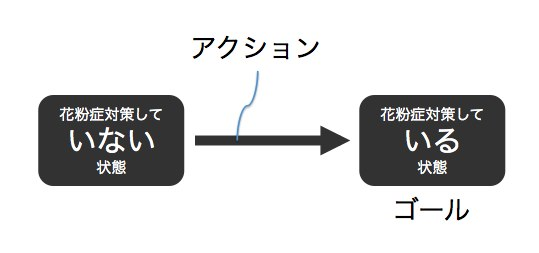
\includegraphics[width=6cm, bb=0 0 350 300]{action_goal.jpg}
\caption{アクションとゴールの例}
\ecaption{Action.}
\label{fig:action_goal}
\end{figure}

\figref{fig:sub_goal}はサブゴールという概念を表現している。「花粉症対策をしていない状態」から「花粉症対策している状態」に移行する間に、別の「花粉症について調べている状態」というものを経由している。


\begin{figure}[tb]
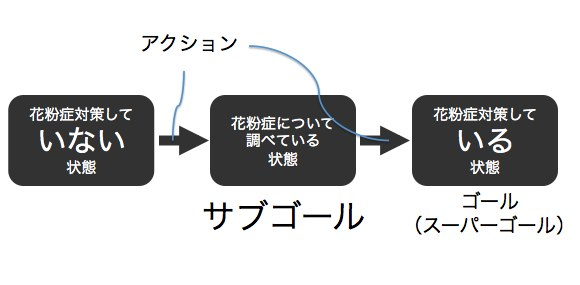
\includegraphics[width=6cm, bb=0 0 450 300]{sub_goal.jpg}
\caption{サブゴールの例}
\ecaption{Action.}
\label{fig:sub_goal}
\end{figure}



\begin{figure}[tb]
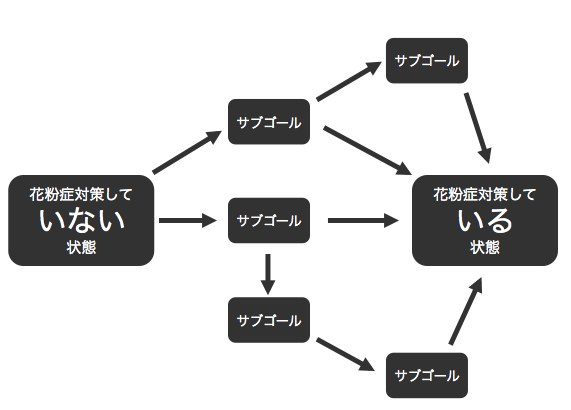
\includegraphics[width=6cm, bb=0 0 450 300]{many_sub_goals.jpg}
\caption{複数のサブゴール}
\ecaption{Action.}
\label{fig:many_sub_goals}
\end{figure}

\begin{itemize}

\item \|タスクとは,遂行すると,目的の一部あるいは全部を達成したことになるアクションである|
\item \|サブタスクとは,タスク同士の関係に着目したとき,「遂行するともう一方のタスクの一部を遂行したことになる行動」である. このとき「もう一方のタスク」はスーパータスクである|
\end{itemize}



\begin{figure}[tb]
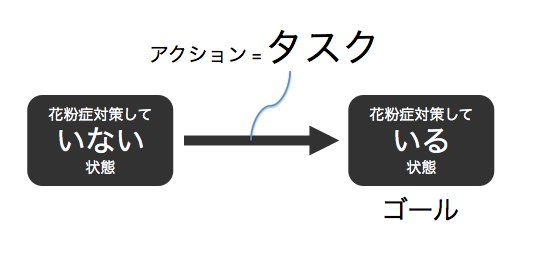
\includegraphics[width=6cm, bb=0 0 450 300]{action_task.jpg}
\caption{タスクの例}
\ecaption{Action Task.}
\label{fig:action_taskl}
\end{figure}

つまり,なんらかのゴールに至るアクションがタスクといえる.ゴールとタスクの関係を\figref{fig:sub_goal}に図示する。

\begin{figure}[tb]
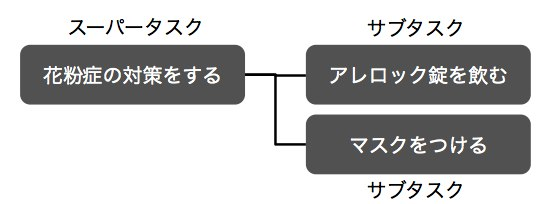
\includegraphics[width=6cm, bb=0 0 400 272]{super_sub.jpg}
\caption{スーパータスクとサブタスクの関係}
\ecaption{Relationships of super task and sub tasks}
\label{fig:super_sub}
\end{figure}

\figref{fig:super_subl}に示すように、サブタスクとスーパータスクは相対的な関係である. あるサブタスクは,別のタスクをサブタスクだとして見ればスーパータスクにあたることもある.

例えば「花粉症対策をする」がスーパータスクだと仮定すると,サブタスクとして「アレロック錠を飲む」,「マスクをつける」といったタスクがあげられる. ここで一段階視点を下げて「アレロック錠を飲む」をスーパータスクと捉えた場合,「診断を受ける」,「薬局を探す」といった行動がサブタスクとなる. 逆の順番でいえば,「薬局に行く」というサブタスクから見たとき「アレロック錠を飲む」はスーパータスクだが,「アレロック錠を飲む」をサブタスクとした場合スーパータスクは「花粉症対策をする」となる.

\begin{figure}[tb]
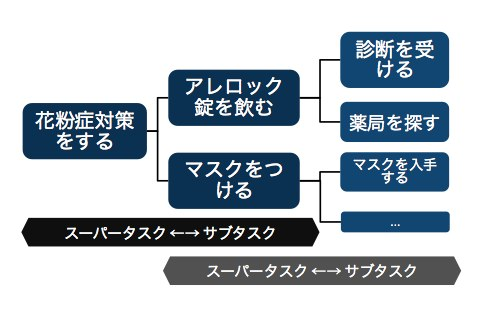
\includegraphics[width=6cm, bb=0 0 350 319]{super_sub_sub.jpg}
\caption{スーパータスクとサブタスクの多重関係}
\ecaption{Multiple relationships of super task and sub tasks}
\label{fig:single}
\end{figure}



ここで注意してほしい点がある. 「花粉症対策をする」のサブタスクとして「薬局に行く」もありうる. 二段階,三段階下のタスクであってもそれはサブタスクなのである. 逆に,「薬局に行く」のスーパータスクとして「花粉症対策をする」がある. つまり,複数段階の連続的な関係と,サブ・スーパーの一段階の関係は両立できる.


%3.2
\subsection{タスク構造}
ある目的を達成するために行動を起こす際,どのような手順で状態が変異するのか整理をする. まず最終的な目的として「花粉対策をする」というタスクがあるとする. これは「花粉症対策をした」というゴールと等価である.

ユーザーは「花粉症対策をしていない」という状態から「花粉症対策をした」という状態に遷移するために必要なアクションを発見しようとする.

「花粉症対策をする」というタスクを遂行する方法はいくつも存在する. 「アレロック錠を飲む」,「マスクをつける」,「医師の診断を受ける」,「薬局に行く」これらすべてが「花粉対策をする」のサブタスクである.

and-or木構造と見なすこともできる. 実際はタスクを遂行する順序やあるタスクを遂行できて初めて遂行可能になるタスクなども存在するため,and-or木構造よりももっと複雑な構造となる.



%4
\section{タスク検索の手法}

%4.1
\subsection{入力}
「(動詞)」または「(名詞)を(動詞)」というクエリを入力する。一例として「花粉症の対策をしたい」という意図でタスク検索を行う場合、「花粉症対策をする」といったクエリが考えられる。入力の例として、以下のものがあげられる。

\begin{itemize}
\item \|花粉症対策をする|
\item \|部屋を掃除する|
\item \|二日酔いを覚ます|
\item \|ダイエットする|
\item \|快眠する|
\item \|おいしいコーヒーを淹れる|
\end{itemize}

以上の例はタスクを動詞として表現したものであるが、実際にはタスクの表現としては動詞以外のものも考えられる。「花粉症対策」「掃除」「快眠」といったものがその例である。

さらに、タスクの表現として、「花粉症対策をした状態」そのものもタスク表現になりうる。たとえがクエリとして「花粉症対策をしている」といった例も考えられる。タスクとは、状態が変化するアクションであるので、状態そのものも「状態に変化する」

状態が本稿ではそれは扱わない。


\subsection{出力}

\begin{itemize}
\item \|立体マスクをつける|
\item \|アレロック錠剤を飲む|
\item \|医師の診断を受ける|
\item \|植物に近寄らない|
\end{itemize}

のように、クエリをスーパータスクとした場合のサブタスクである「(名詞)(助詞)(動詞)」の文章が出力される。



%5
\section{評価}
実験を行った.

%5.1
\subsection{実験の手法}
ベースラインとして、単純な言語パターンを用いてサブタスク検索を行うシステムを使う。

ベースラインは上位にランクづけされたページをスクリプティングして、タスクに使われることの多い「使う」「おすすめ」といった単語を見つけるとその

\begin{enumerate}
\item \|クエリを形態素解析して名詞と動詞を抽出する|
\item \|名詞と動詞をキーワードにした新たなクエリを作成する|
\item \|Google Cusom Search APIを使い,新たなクエリでWeb検索する|
\item \|上位100件のページを取得する|
\item \|ページ内から「使う」「おすすめ」といったタスクに使われる可能性の高い単語を含む文章を発見する|
\end{enumerate}

以上の手順で,タスクと推測できる文を発見する.




\begin{itemize}
\item \|花粉症対策をする|
\item \|部屋を掃除する|
\item \|二日酔いを覚ます|
\item \|ダイエットする|
\item \|快眠する|
\item \|おいしいコーヒーを淹れる|
\end{itemize}


以上のクエリから、サブタスクを探す。

理想的なサブタスクとしては、たとえば「部屋を掃除する」をクエリとした場合、

\begin{itemize}
\item \|掃除機をかける|
\item \|パナソニックの掃除機を買う|
\item \|家事代行に依頼する|
\item \|友達に掃除を頼む|
\item \|ルンバを使う|
\item \|お茶の出がらしをまく|
\end{itemize}

といったサブタスクが出力されれば理想的である。ここで注意していただきたいことがある。「掃除機をかける」と「パナソニックの掃除機を買う」は並列したタスクではなく、「パナソニックの掃除機を買って、それから掃除機をかける」という連続的関係にあるタスクかもしれない。しかし本研究では連続したタスクであっても、別個のタスクとして扱う。よって、「掃除機をかける」と「パナソニックの掃除機を買う」は別のタスクだと判断する。


\begin{figure}[tb]
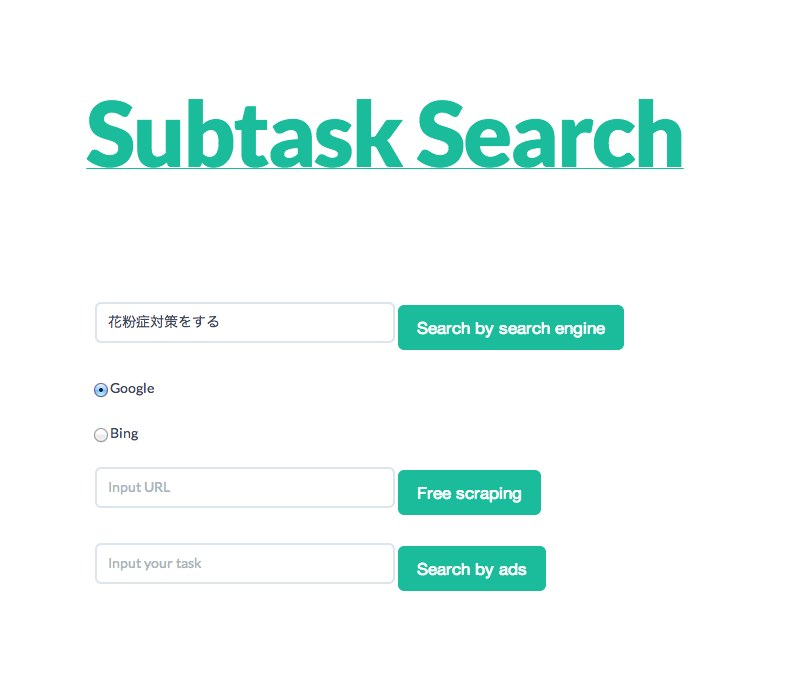
\includegraphics[width=6cm, bb=0 0 550 719]{base_line1.jpg}
\caption{ベースライン}
\ecaption{Multiple relationships of super task and sub tasks}
\label{fig:single}
\end{figure}


%5.2
\subsection{実験の結果}

ベースラインの手法では,「医療機関や薬剤師に相談する」「加湿器を使う」「花粉症の市販薬を選ぶ」といったタスクを発見できる.しかし「むずむずするときに飲んでみてください」といったタスクの断片や、そもそもタスクではない「設定してください」といった文も発見してしまう。

\begin{figure}[tb]
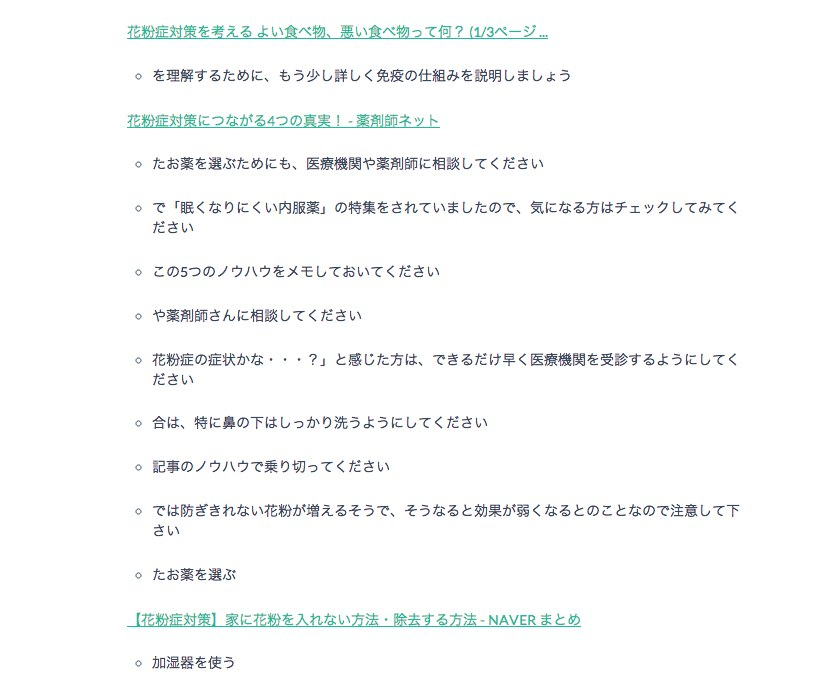
\includegraphics[width=6cm, bb=0 0 550 719]{base_line3.jpg}
\caption{ベースラインの結果}
\ecaption{Multiple relationships of super task and sub tasks}
\label{fig:single}
\end{figure}



\begin{table}[tb] 
\caption{花粉症対策の方法タスク検索} 
\ecaption{An Example of Table.}
\label{tab:example}
\hbox to\hsize{\hfil
\begin{tabular}{l|lll}\hline\hline
& 発見数 & 正解数 & 正解率 \\\hline
ベースライン &	161 & item 2,1 & ---\\
row4 &	item 1,4 & item 2,4 & item 3,4 \\\hline
\end{tabular}\hfil}
\end{table}



%6
\section{考察}


%7
\section{結論}




\begin{thebibliography}{10}


\bibitem{yamatake}
The Widwom of Advertisers: Mining Subgoals via Query Clustering
\urlj{http://research.microsoft.com/en-us/people/tesakai/cikm2012yamamoto.pdf}
(2012.11.02).

\bibitem{hassan}
Task Tours: Helping Users Tackle Complex Search Tasks:
Ahmed Hassan,Ryen W. White
\urlj{http://research.microsoft.com/pubs/178868/HassanCIKM2012.pdf}

\bibitem{tamugi}
Tamugi search:
\urlj{http://somewhere.pdf}




\end{thebibliography}



\begin{biography}
\profile{m}{加藤 龍}{1988年生.2012年京都大学農学部卒. 2012年同大学院情報学研究科入学}
%
\end{biography}



\end{document}
